\section*{A wild \lstinline'struct' appears%
\TAGS{memory-model, pointer, struct}}

Suppose we have the following in a file:

\begin{tabular}{l r}
    {\begin{lstlisting}[numbers=left]
struct X {
  int a;
  struct Y* b; };

struct Y {
  int* a;
  int b;
  struct X* c; };

int main() {
  struct X* foo = alloc(struct X);
  struct Y* bar = alloc(struct Y);

  foo->b = bar;
  bar->c = foo;
  bar->c->a = 15;
  foo->b->a = alloc(int);
  *(bar->a) = foo->a * 8 + 2;
  foo->b->b = 1000 * foo->a + *(foo->b->a);

  return 0;
}
    \end{lstlisting}}
& \raisebox{-30ex}{%
  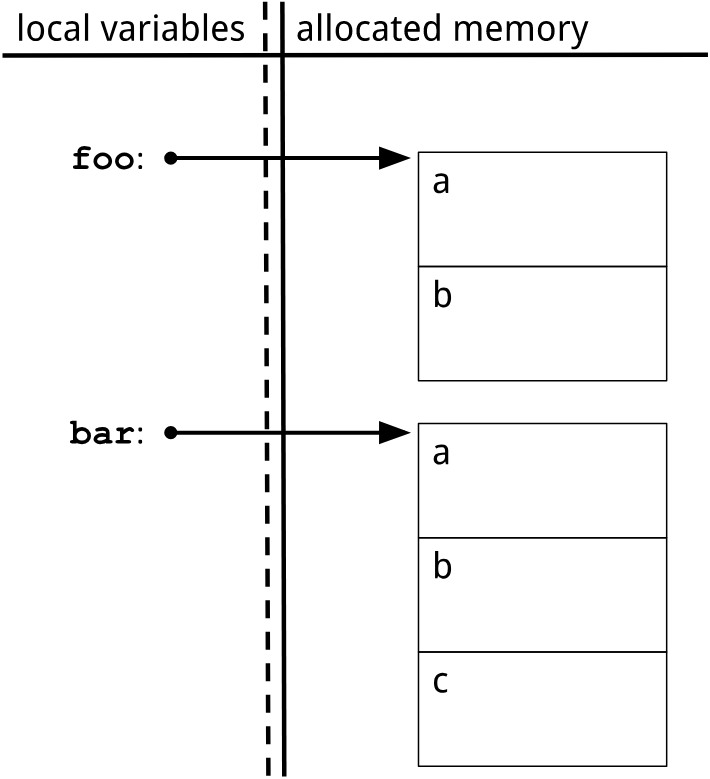
\includegraphics[width=0.35\textwidth]{\img/structs_with_table.png}}
\end{tabular}

\checkpoint*{\TAGS{memory-model, pointer, struct}}

Fill out the state of the memory.  What's the value of \lstinline'bar->b'?
(For your own sanity, draw a picture!)

\begin{solution}

  foo->a = 15; \\
  foo->b = bar;\\

  bar->a points to a new block of allocated memory containing 122\\
  bar->b = 15122;\\
  bar->c = foo;
\end{solution}
